\pdfsuppresswarningpagegroup=1
\section{Results - data not fitted}

We look at the statistical estimators for data which was not fitted, we split
that data into two groups: new processes and old processes. Since we are looking
at closure test data which has not been fitted, we ignore any double counting
in the data - for example jet measurements with different jet radii,
or different single top distributions.

\subsection{Out of sample data, New processes}

\begin{center}
    \resizebox{0.6\textwidth}{!}{\begin{tabular}{llll}
        \toprule
        {} & Training fraction & C-factors & Other fields \\
        Dataset                                &                   &           &              \\
        \midrule
        ATLASPHT12                             &                 - &       QCD &            - \\
        ATLASPHT15                             &                 - &       QCD &            - \\
        ATLAS\_SINGLETOP\_TCH\_R\_7TEV             &                 - &       QCD &            - \\
        ATLAS\_SINGLETOP\_TCH\_DIFF\_7TEV\_T\_PT     &                 - &       QCD &            - \\
        ATLAS\_SINGLETOP\_TCH\_DIFF\_7TEV\_T\_RAP    &                 - &       QCD &            - \\
        ATLAS\_SINGLETOP\_TCH\_DIFF\_7TEV\_TBAR\_PT  &                 - &       QCD &            - \\
        ATLAS\_SINGLETOP\_TCH\_DIFF\_7TEV\_TBAR\_RAP &                 - &       QCD &            - \\
        ATLAS\_SINGLETOP\_TCH\_R\_8TEV             &                 - &       QCD &            - \\
        ATLAS\_SINGLETOP\_TCH\_DIFF\_8TEV\_T\_PT     &                 - &       QCD &            - \\
        ATLAS\_SINGLETOP\_TCH\_DIFF\_8TEV\_T\_RAP    &                 - &       QCD &            - \\
        ATLAS\_SINGLETOP\_TCH\_DIFF\_8TEV\_TBAR\_PT  &                 - &       QCD &            - \\
        ATLAS\_SINGLETOP\_TCH\_DIFF\_8TEV\_TBAR\_RAP &                 - &       QCD &            - \\
        ATLAS\_SINGLETOP\_TCH\_R\_13TEV            &                 - &       QCD &            - \\
        ATLAS\_2JET\_7TEV\_R06                    &                 - &  QCD, EWK &            - \\
        ATLAS\_2JET\_7TEV\_R04                    &                 - &  QCD, EWK &            - \\
        ATLAS\_WP\_JET\_8TEV\_PT                   &                 - &       QCD &            - \\
        ATLAS\_WM\_JET\_8TEV\_PT                   &                 - &       QCD &            - \\
        ATLAS\_WP\_JET\_8TEV\_PTJ                  &                 - &       QCD &            - \\
        CMS\_SINGLETOP\_TCH\_TOT\_7TEV             &                 - &       QCD &            - \\
        CMS\_SINGLETOP\_TCH\_R\_8TEV               &                 - &       QCD &            - \\
        CMS\_SINGLETOP\_TCH\_R\_13TEV              &                 - &       QCD &            - \\
        CMS\_2JET\_7TEV                          &                 - &  QCD, EWK &            - \\
        CMS\_2JET\_3D\_8TEV                       &                 - &  QCD, EWK &            - \\
        \bottomrule
        \end{tabular}}
\end{center}

\subsection{Out of sample data, Old process}

\begin{center}
    \resizebox{0.6\textwidth}{!}{\begin{tabular}{llll}
        \toprule
        {} & Training fraction & C-factors & Other fields \\
        Dataset                          &                   &           &              \\
        \midrule
        HERACOMB\_SIGMARED\_C              &                 - &         - &            - \\
        HERACOMB\_SIGMARED\_B              &                 - &         - &            - \\
        ATLAS\_1JET\_8TEV\_R06              &                 - &  QCD, EWK &            - \\
        ATLAS\_1JET\_8TEV\_R04              &                 - &  QCD, EWK &            - \\
        ATLAS\_TOPDIFF\_DILEPT\_8TEV\_TTM    &                 - &       QCD &            - \\
        ATLAS\_TOPDIFF\_DILEPT\_8TEV\_TTRAP  &                 - &       QCD &            - \\
        ATLASWZRAP11CF                   &               0.5 &       QCD &            - \\
        ATLAS\_WZ\_TOT\_13TEV               &               0.5 &       QCD &            - \\
        CMS\_1JET\_8TEV                    &                 - &  QCD, EWK &            - \\
        CMS\_TTBAR\_2D\_DIFF\_PT\_TRAP\_NORM   &                 - &       QCD &            - \\
        CMS\_TTBAR\_2D\_DIFF\_MTT\_TRAP\_NORM  &                 - &       QCD &            - \\
        CMS\_TTBAR\_2D\_DIFF\_MTT\_TTRAP\_NORM &                 - &       QCD &            - \\
        CMSTTBARTOT5TEV                  &                 - &       QCD &            - \\
        CMS\_TTB\_DIFF\_13TEV\_2016\_LJ\_TPT   &                 - &       QCD &            - \\
        CMS\_TTB\_DIFF\_13TEV\_2016\_LJ\_TRAP  &                 - &       QCD &            - \\
        CMS\_TTB\_DIFF\_13TEV\_2016\_LJ\_TTRAP &                 - &       QCD &            - \\
        CMS\_TTB\_DIFF\_13TEV\_2016\_LJ\_TTM   &                 - &       QCD &            - \\
        CMS\_TTB\_DIFF\_13TEV\_2016\_2L\_TPT   &                 - &       QCD &            - \\
        CMS\_TTB\_DIFF\_13TEV\_2016\_2L\_TRAP  &                 - &       QCD &            - \\
        CMS\_TTB\_DIFF\_13TEV\_2016\_2L\_TTRAP &                 - &       QCD &            - \\
        CMS\_TTB\_DIFF\_13TEV\_2016\_2L\_TTM   &                 - &       QCD &            - \\
        LHCB\_Z\_13TEV\_DIMUON              &                 - &       QCD &            - \\
        LHCB\_Z\_13TEV\_DIELECTRON          &                 - &       QCD &            - \\
        \bottomrule
        \end{tabular}}
\end{center}

\subsection{Data space estimators}

First we show $\sqrt{\frac{\eshift{\bias}}{\eshift{\var}}}$ by experiment for data
not included in the fit, but old processes.

\begin{center}
    \begin{tabular}{lrr}
        \toprule
        {} &  $\ndata$ &  $\sqrt{\frac{\eshift{\bias}}{\eshift{\var}}}$ \\
        experiment &        &                      \\
        \midrule
        HERACOMB   &     63 &                 1.60 \\
        ATLAS      &    371 &                 0.76 \\
        CMS        &    310 &                 0.87 \\
        LHCb       &     35 &                 0.83 \\
        Total      &    779 &                 0.89 \\
        \bottomrule
        \end{tabular}
\end{center}

Next we show the same estimator, $\sqrt{\frac{\eshift{\bias}}{\eshift{\var}}}$, by
experiment for data not included in the fit, new processes

\begin{center}
    \begin{tabular}{lrr}
        \toprule
        {} &  $\ndata$ &  $\sqrt{\frac{\eshift{\bias}}{\eshift{\var}}}$ \\
        experiment &        &                      \\
        \midrule
        ATLAS      &    374 &                 1.00 \\
        CMS        &    179 &                 0.81 \\
        Total      &    553 &                 0.90 \\
        \bottomrule
        \end{tabular}
\end{center}

Now we compare the measured $\xi_{1\sigma}$ and estimated $\xi_{1\sigma}$ by experiment
for data not included in the fit, old processes. To estimate $\xi_{1\sigma}$
we we take $\sqrt{\frac{\eshift{\bias}}{\eshift{\var}}}$ and substitute into
eq. \eqref{eq:expectedxi}, assuming that $\frac{\sigma_i}{\modelstd_i}$ is
constant across datapoints and equal to $\sqrt{\frac{\eshift{\bias}}{\eshift{\var}}}$.

\begin{center}
    \begin{tabular}{lrrr}
        \toprule
        {} &  $\ndata$ &  measured $\xi_{1\sigma}$ &  estimated $\xi_{1\sigma}$ from bias/variance \\
        experiment &        &                           &                                                  \\
        \midrule
        HERACOMB   &     63 &                      0.46 &                                             0.47 \\
        ATLAS      &    371 &                      0.77 &                                             0.81 \\
        CMS        &    310 &                      0.69 &                                             0.75 \\
        LHCb       &     35 &                      0.78 &                                             0.77 \\
        Total      &    779 &                      0.72 &                                             0.74 \\
        \bottomrule
        \end{tabular}
\end{center}


Similarly, we compare the same estimators $\xi_{1\sigma}$ and estimated
$\xi_{1\sigma}$ by experiment for data not included in the fit, new processes.

\begin{center}
    \begin{tabular}{lrrr}
        \toprule
        {} &  $\ndata$ &  measured $\xi_{1\sigma}$ &  estimated $\xi_{1\sigma}$ from bias/variance \\
        experiment &        &                           &                                                  \\
        \midrule
        ATLAS      &    374 &                      0.66 &                                             0.69 \\
        CMS        &    179 &                      0.76 &                                             0.78 \\
        Total      &    553 &                      0.69 &                                             0.73 \\
        \bottomrule
        \end{tabular}
\end{center}


We now show $\xi_{1\sigma}^{i}$ for data which was not fitted, old processes. Split
up by experiment, each scatter point is $\xi_{1\sigma}^{i}$ for a given datapoint
in the basis which diagonalises the respective experimental covariance matrix.

\begin{figure}[!b]
    \centering
    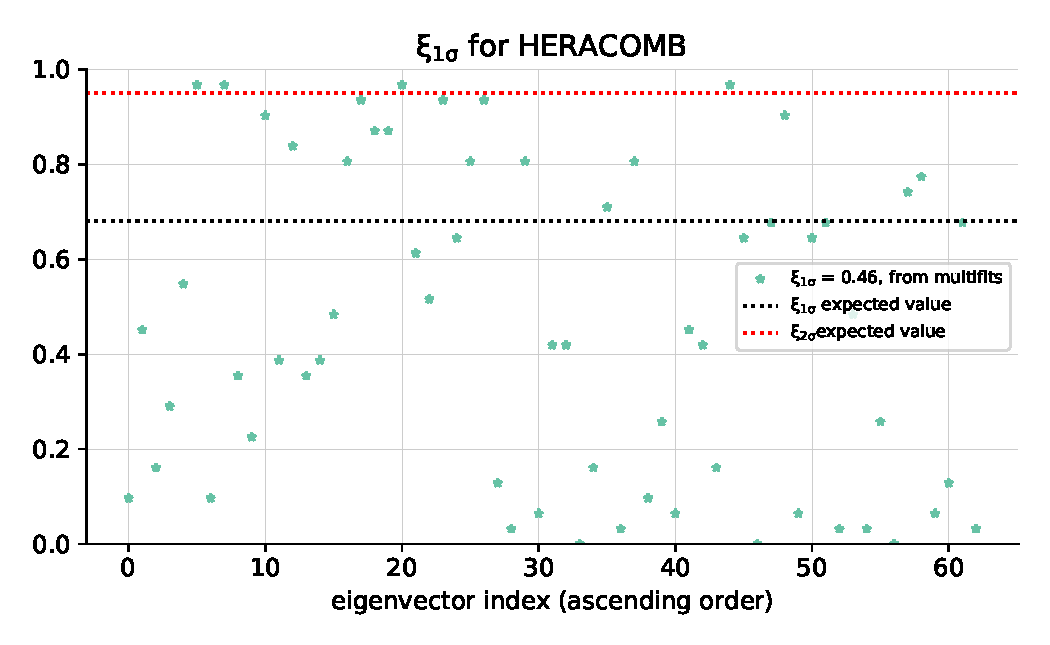
\includegraphics[width=0.6 \textwidth]{out_oldproc_hera_xi.pdf}
    \caption{$\xi_{1\sigma}^{i}$ for HERA datasets which were not fitted
    but are old processes, in the basis which diagonalises the experimental
    covariance matrix. The dashed black line shows the ideal result, 0.68, when
    the spread of replica theory predictions around the mean is equal to the
    spread of the expectation of theory predictions across replicas around the
    underlying law. The dashed red line shows the ideal result for the $2\sigma$
    contour for reference.}
    \label{fig:outoldheraxi}
\end{figure}

\begin{figure}[ht]
    \centering
    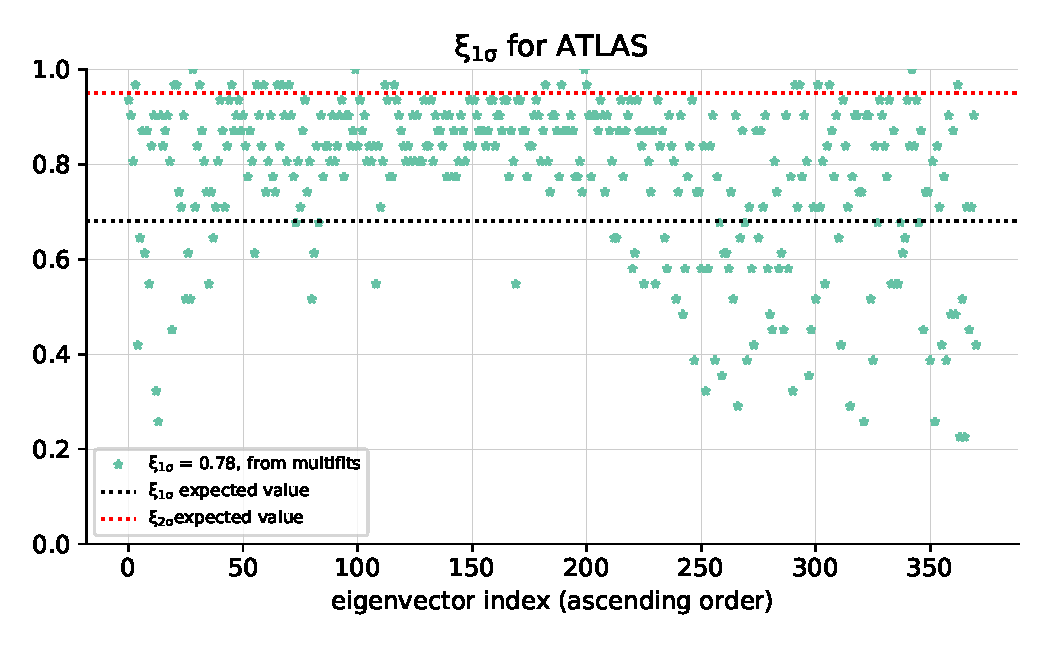
\includegraphics[width=0.6 \textwidth]{out_oldproc_atlas_xi.pdf}
    \caption{$\xi_{1\sigma}^{i}$ for ATLAS datasets which were not fitted
    but are old processes, in the basis which diagonalises the experimental
    covariance matrix. The dashed black line shows the ideal result, 0.68, when
    the spread of replica theory predictions around the mean is equal to the
    spread of the expectation of theory predictions across replicas around the
    underlying law. The dashed red line shows the ideal result for the $2\sigma$
    contour for reference.}
    \label{fig:outoldatlasxi}
\end{figure}

\begin{figure}[ht]
    \centering
    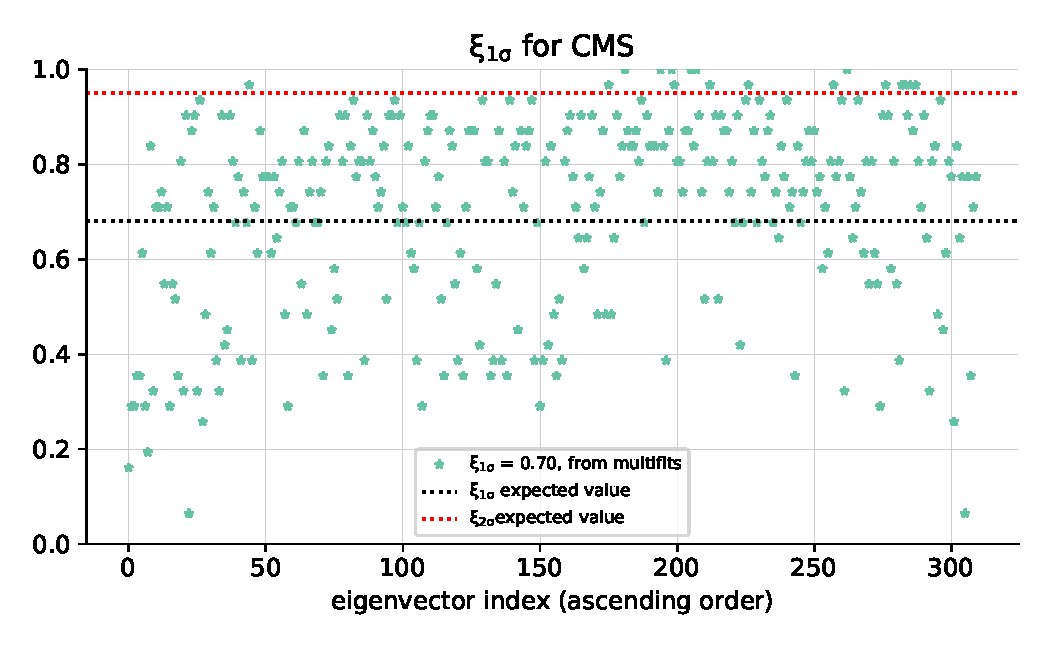
\includegraphics[width=0.6 \textwidth]{out_oldproc_cms_xi.pdf}
    \caption{$\xi_{1\sigma}^{i}$ for CMS datasets which were not fitted
    but are old processes, in the basis which diagonalises the experimental
    covariance matrix. The dashed black line shows the ideal result, 0.68, when
    the spread of replica theory predictions around the mean is equal to the
    spread of the expectation of theory predictions across replicas around the
    underlying law. The dashed red line shows the ideal result for the $2\sigma$
    contour for reference.}
    \label{fig:outoldcmsxi}
\end{figure}

\begin{figure}[ht]
    \centering
    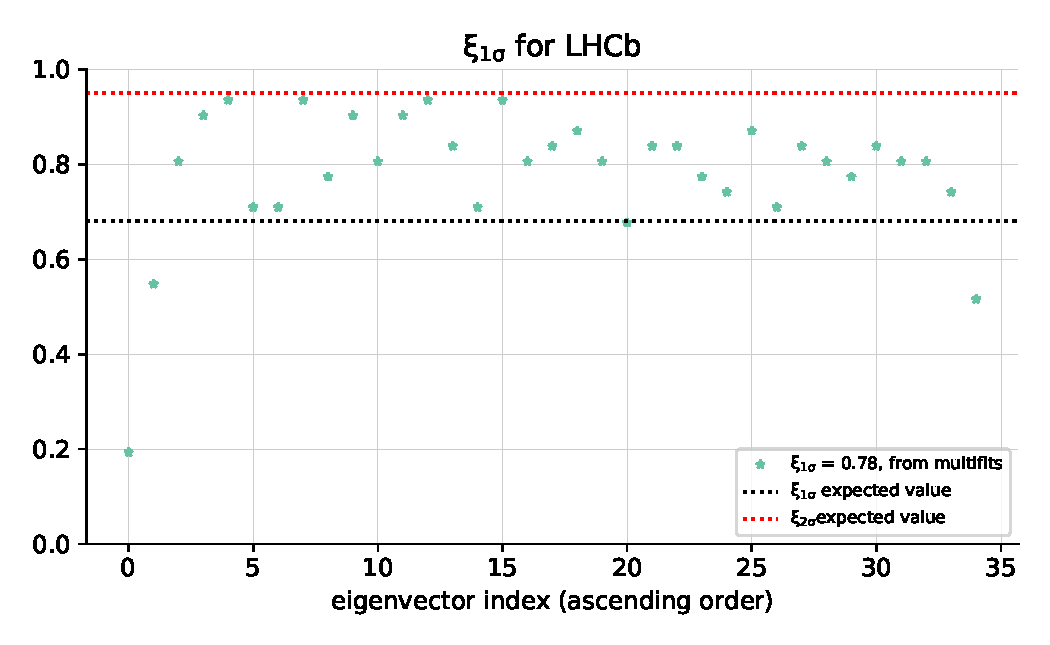
\includegraphics[width=0.6 \textwidth]{out_oldproc_lhcb_xi.pdf}
    \caption{$\xi_{1\sigma}^{i}$ for LHCb datasets which were not fitted
    but are old processes, in the basis which diagonalises the experimental
    covariance matrix. The dashed black line shows the ideal result, 0.68, when
    the spread of replica theory predictions around the mean is equal to the
    spread of the expectation of theory predictions across replicas around the
    underlying law. The dashed red line shows the ideal result for the $2\sigma$
    contour for reference.}
    \label{fig:outoldlhcbxi}
\end{figure}

Now the corresponding plots for data which was not fitted, new processes.

\begin{figure}[ht]
    \centering
    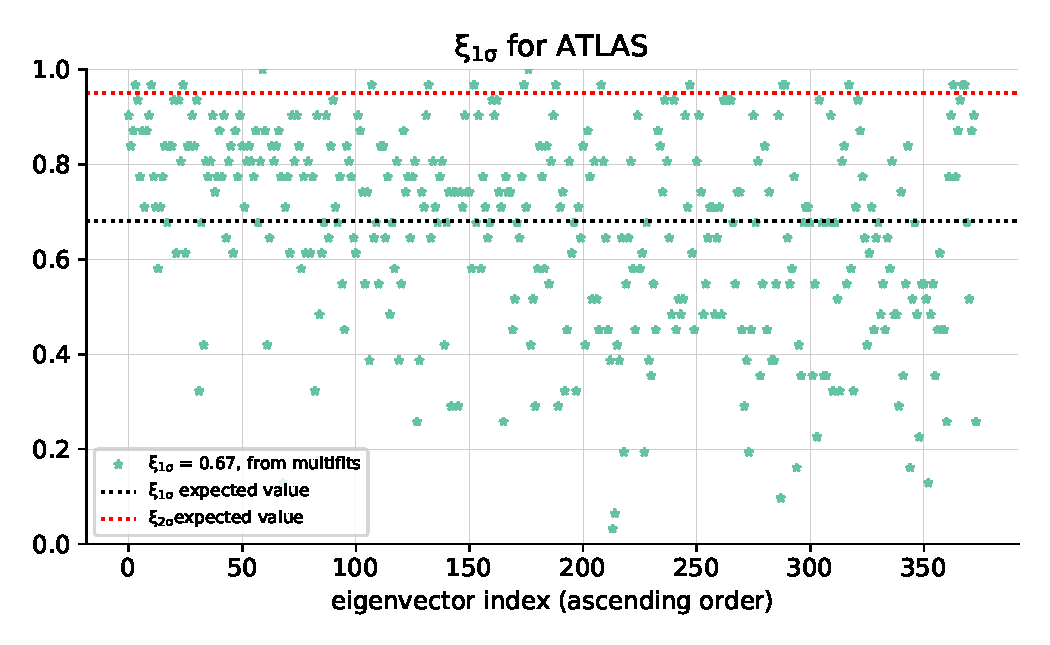
\includegraphics[width=0.6 \textwidth]{out_newproc_atlas_xi.pdf}
    \caption{$\xi_{1\sigma}^{i}$ for ATLAS datasets which were not fitted
    and are new processes, in the basis which diagonalises the experimental
    covariance matrix. The dashed black line shows the ideal result, 0.68, when
    the spread of replica theory predictions around the mean is equal to the
    spread of the expectation of theory predictions across replicas around the
    underlying law. The dashed red line shows the ideal result for the $2\sigma$
    contour for reference.}
    \label{fig:outnewatlasxi}
\end{figure}

\begin{figure}[ht]
    \centering
    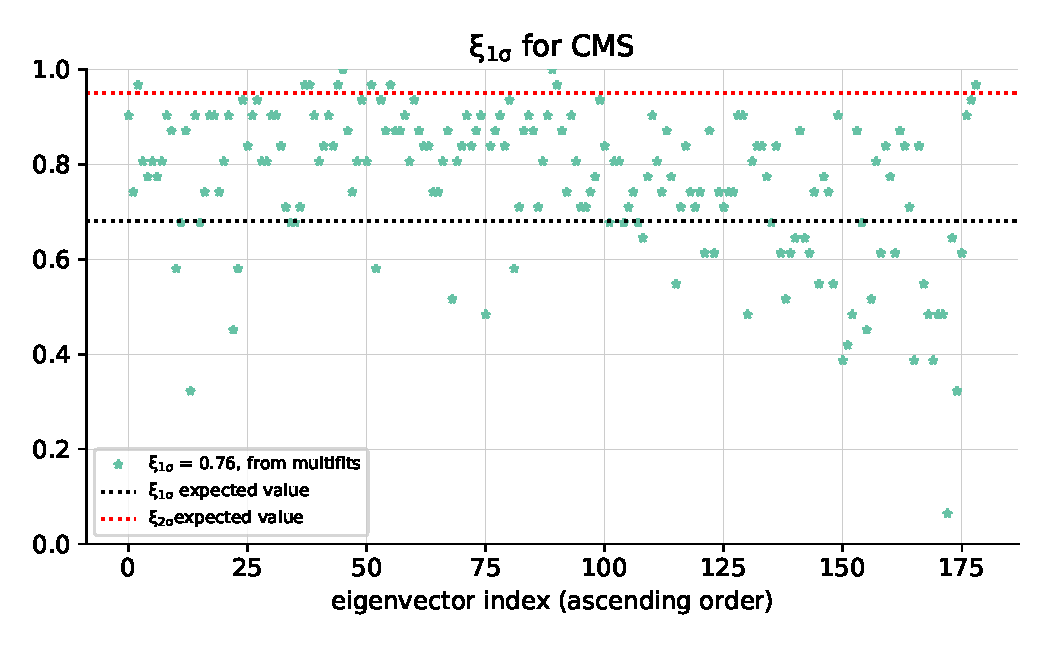
\includegraphics[width=0.6 \textwidth]{out_newproc_cms_xi.pdf}
    \caption{$\xi_{1\sigma}^{i}$ for CMS datasets which were not fitted
    and are new processes, in the basis which diagonalises the experimental
    covariance matrix. The dashed black line shows the ideal result, 0.68, when
    the spread of replica theory predictions around the mean is equal to the
    spread of the expectation of theory predictions across replicas around the
    underlying law. The dashed red line shows the ideal result for the $2\sigma$
    contour for reference.}
    \label{fig:outnewcmsxi}
\end{figure}

There is no noticeable trend between new and old processes with the data which
was not fitted. Potentially we can condense the above plots significantly. At
least into just 4 plots (by experiment). The results would change slightly
due to the basis being different.
